\chapter{Flexible Tree Matching}
One problem of the standard tree edit distance is the strict requirement regarding the tree parent-to-child relationship within an ordered tree, the so called hierarchy, and ordering among siblings. If a node gets mapped while computing the tree edit distance, its children have to get mapped to some descendants of this mapped node. In some domains, the most appropriate matching may not follow these requirements. One of these domains is the DOM (Document Object Model) of a website. A standard HTML-based website can easily be structured according to the respective tags. Take a look at the website in Figure~\ref{fig:website_0} and the its HTML-code in Listing~\ref{lst:DOM0}. 
\begin{figure}[!h]
    \centering
        
\includegraphics[width=0.60\textwidth]{figures/DOM_website.png}
        \caption{The example website.}
        \label{fig:website_0}
\end{figure} 
\lstinputlisting[language=Html, caption=Html code of DOM example, label=lst:DOM0]{figures/DOM_0.html}

The DOM-tree of the example website is intuitively clear: The outermost tag, the $<$html$>$-tag, is the tree's root. The root's children are the $<$head$>$-tag and the $<$body$>$-tag and so on. This leads to complete DOM-tree illustrated in Figure~\ref{fig:DOM_0}.
\begin{figure}[!h]
    \centering
        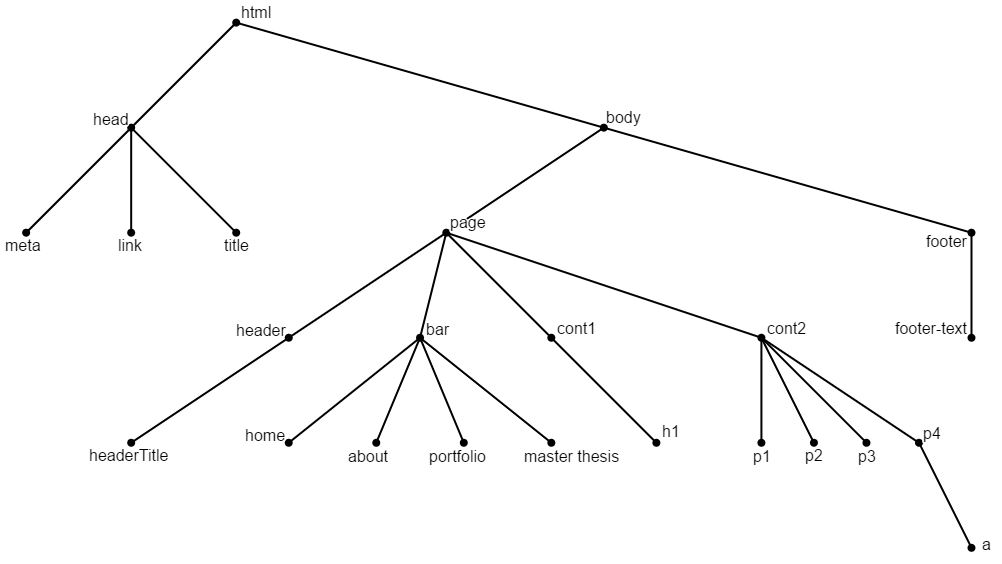
\includegraphics[width=1\textwidth]{figures/DOM_0.jpg}
        \caption{Complete DOM-tree of the example website.}
        \label{fig:DOM_0}
\end{figure}
\\
Intuitively, any small change to the website should not lead to a big distance between the two DOM-trees. Suppose one changes the order of the buttons in the header menu as well as moving one of these buttons into the content area of the website as seen in Figure~\ref{fig:website_1}. The website and its functionalities remain quite similar, but it would take about three deletions and four insertions to end up with the new DOM-tree. Obviously it would be cheaper to delete the whole header menu and therefore reduce the functionality of the website. 
\begin{figure}[!h]
    \centering
        
\includegraphics[width=0.60\textwidth]{figures/DOM_website_1.png}
        \caption{Small changes to the website should not affect the distance of the respective DOM-trees.}
        \label{fig:website_1}
\end{figure} 

This kind of issue arises frequently in the context of comparing tree models. Flexible tree matching models have been introduced in an effort to appropriately handle the above mentioned issues. Instead of requiring strict left-to-right ordering and hierarchy conditions, one may relax them by introducing costs to penalize the violation of this type of requirements. Kumar et al.~\cite{Kum} developed an algorithm that matches nodes with similar labels and penalizes edges that break up sibling groups or violate the hierachy. In the example above, moving the button from header menu into the content is such a violation of the hierarchy, because a node gets shifted into another subtree. A violation of this kind needs to have some costs associated to it, but it should definitely be cheaper than deleting the subtree and inserting it again in some other place.\\
Finding the minimum flexible tree edit distance can be reduced to finding a minimum cost matching in a flexible cost model. Kumar et al. showed that finding the flexible tree edit distance is strongly $\mathcal{NP}$-complete. This implies that there are no efficient algorithms to compute the minimum flexible tree edit distance. However, there are some approximating heuristics.\\
This chapter is based on the previously cited paper by Kumar et al. 

\section{The Model for the Flexible Tree Edit Distance}
\begin{defin}\label{def:graph_fted}
Let $T_1$ and $T_2$ be two rooted ordered labelled trees with a set of labels $\Sigma$. We define a complete bipartite graph $G_{T_1,T_2}$ on the following set of nodes:\\
$$G := (\{V(T_1)\cup \otimes_1\} \dot{\cup} \{V(T_2)\cup \otimes_2\}, E(G_{T_1,T_2}))$$
Hence the edge set $E(G_{T_1,T_2})$ is defined as the set: 
$$E(G_{T_1,T_2}):=\{\{v_1,v_2\} \;|\; v_i \in\{V(T_i)\cup \otimes_i\}\text{ for }i =1,2\}.$$
The nodes $\otimes_i$ are so called \textit{no-match} nodes.
\end{defin}
\begin{rem}
Every edge $e=\{v_1,v_2\}\in E(G_{T_1,T_2})$ represents matching a node $v_1$ to a node $v_2$. If $v_2=\otimes_2$, the edge $e$ would represent the deletion of $v_1$, since $v_1$ was not matched to any node from the tree $T_2$. An analogous statement holds for an edge $\{\otimes_1,v_2\}$. 
\end{rem}
\begin{defin}
Let $T_1$ and $T_2$ be two rooted ordered labelled trees with a set of labels $\Sigma$ and the graph $G_{T_1, T_2}$ be given. We call a set of edges $M \subseteq E(G_{T_1,T_2})$ a \textit{flexible matching}, if the following statements are true:
\begin{enumerate}
\item $\forall v_1 \in \, V(T_1): \exists !v_2 \in \{V(T_2)\cup \otimes_2\} \, \text{s.t.:} \quad (v_1, v_2) \in E(G_{T_1,T_2})$
\item $\forall v_2 \in \, V(T_2): \exists !v_1 \in \{V(T_1)\cup \otimes_1\} \, \text{s.t.:} \quad (v_1, v_2) \in E(G_{T_1,T_2})$
\end{enumerate}
We call the set of all flexible matchings $M_{T_1, T_2}$
\end{defin}
\begin{rem}
Note, that the no-match nodes do not have any restrictions on them. A no-match node may be a part of $0$ edges or it may be arbitrarily often matched. 
\end{rem}
Every edge $e \in E(G_{T_1,T_2})$, $e \in V(T_1) \times V(T_2)$ is assigned some cost function $c(e)$:
\begin{equation}\label{eq:edgeCost}
c(e) = c_r(e) + c_a(e) + c_s(e).
\end{equation} 
The exact definitions follow later. In short terms, these three summands represent the costs that we mentioned earlier in this chapter: $c_r$ represents the costs of relabelling a node, $c_a$ penalizes violations of ancestry relationships and $c_s$ punishes broken up sibling groups. All the other edges, namely the ones connecting tree nodes with no-match nodes, have a fixed constant cost $w_n$, only depending on the number of nodes in the trees.

Suppose that $v \in V(T_1)$ and $w \in V(T_2)$ and let $e:=\{v,w\}\in E$. The costs for relabelling $e$, i.e. $c_r(e)$, only depend on the nodes $v$ and $w$ themselves. They are fixed for every edge and are known before starting to match nodes. $c_a(e)$ and $c_s(e)$ on the other hand may depend on the choice of the flexible matching $M$. To be more precise the costs $c_a(\{v,w\})$ are linearly dependent on the number of children of $v$ that do not get mapped onto children of $w$. Define $M(v)\in \{T_2\cup\otimes_2\}$ to be the node that $v$ is mapped onto according to the flexible matching $M$ and suppose that $M(v) \neq \otimes_2$. Moreover, define $C(v) \subset T_1$ to be the set of children of node $v$. Then we can define $V(v)$ to be the set of children of $v$ that violate the ancestry condition, i.e.:
\begin{equation}
V(v) := \{v' \in C(v)\;|\;M(v') \in T_2 \setminus C(M(v))\}
\end{equation}
As stated previously, the cost function $c_a(e)$ is linearly dependent on the sizes of the sets $V(v)$ and $V(w)$ with some constant factor $\omega_a$:
\begin{equation}\label{eq:fted_ca}
c_a(\{v,w\}) := \omega_a (|V(v)| + |V(w)|)
\end{equation}
\begin{figure}[b!]
    \centering
        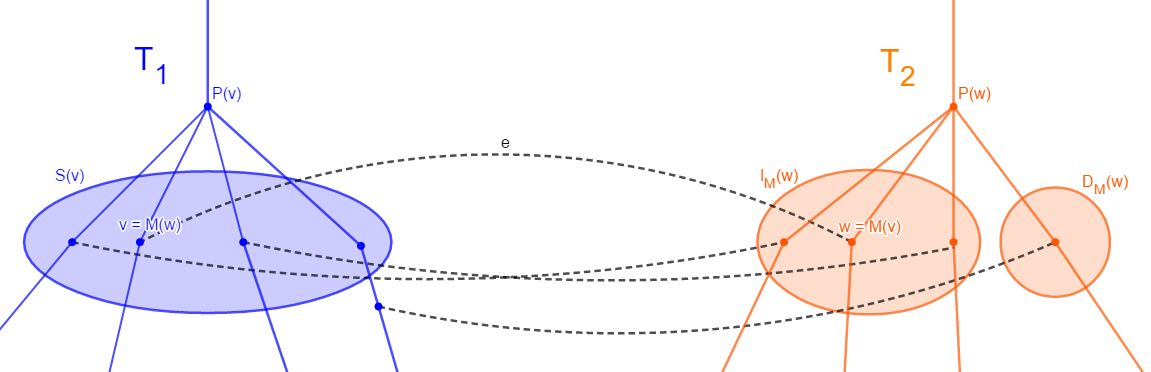
\includegraphics[width=\textwidth]{figures/Treeconcepts_flexible_tree_matching.png}
        \caption{A visual representation of the above described tree concepts.}
        \label{fig:treeConcepts}
\end{figure}
We need further tree related concepts before we can define the cost function $c_s(e)$ in a straight forward way. Therefore $P(v) \in T_1$ is defined as the parent of the node $v$ and $S(v):=C(P(v))$ is the sibling group of $v$. If $v$ is the root of the tree, then $P(v)$ does not exist and $S(v):=\{v\}$. Note that the sibling group $S(v)$ always contains the node $v$ itself and thus is not empty. For a matching $M$, we define the sibling-invariant subset of $I_M(v)$ of $v$, to be the siblings of $v$ which are mapped into the same sibling group as $v$:
\begin{equation}
I_M(v) = \{v' \in S(v)\;|\;M(v') \in S(M(v))\}
\end{equation}
Accordingly the sibling-divergent subset of $v$, $D_M(v)$, are the siblings of $v$ which are mapped to a node in $T_2 \setminus S(M(v))$:
\begin{align}
D_M(v) :&= \{v' \in S(v)\;|\;M(v') \in T_2 \setminus S(M(v))\} \\
		&= \{v' \in S(v) \setminus I_M(v)\;|\;M(v') \neq \otimes_2\}
\end{align}
Finally, we define the set of distinct sibling families to be the set of all sibling groups, that the siblings of $v$ map into:
\begin{equation}
F_M(v) = \bigcup_{v' \in S(v)} P(M(v'))
\end{equation}
Now we can define the costs for sibling group violations depending on a constant $\omega_s$:
\begin{equation}\label{eq:fted_cs}
c_s(\{v,w\},M) := \omega_s (\frac{|D_M(v)|}{|I_M(v)||F_M(v)|} + \frac{|D_M(w)|}{|I_M(w)||F_M(w)|})
\end{equation}
One can show, that the costs $c_s(\{v,w\},M)$ increase, if a node in the sibling group of $v$ or $w$ gets reassigned to some node outside of the corresponding sibling group.

\begin{defin}
Let $T_1$, $T_2$ be two rooted ordered trees. Let $G := (\{V(T_1)\cup \otimes_1\} \dot{\cup} \{V(T_2)\cup \otimes_2\}, E)$ be a graph as defined above. Furthermore let constants $\omega_n$, $\omega_a$, $\omega_s$ and the relabelling function $c_r(e)$ be given.\\
Let $M^* \in M_{T_1, T_2}$ be a flexible matching that covers each node $v \in T_i$, $i \in \{1,2\}$ exactly once and that fulfills the following equation:
$$c(M^*) := \sum_{e^* \in M^*} \, c(e^*) = \min_{M \in M_{T_1, T_2}} \sum_{e \in M} \, c(e)
$$
where $c(e)$ is defined as described in the Equations (\ref{eq:edgeCost}),(\ref{eq:fted_ca}),(\ref{eq:fted_cs}). Then we call $c(M^*)$ the \textit{flexible tree edit distance}.
\end{defin}

\section{Approximation and Conclusion}
As mentioned in the introduction of this section, computing the flexible tree edit distance is $\mathcal{NP}$-hard. There is a short and elegant proof for that, based on a reduction of the 3-partition problem to the flexible tree matching problem. Once again you can find the details in the paper of Kumar et al~\cite{Kum}. Hence, there exists no efficient algorithm that computes the flexible tree matching to optimality. But there are stochastic optimization algorithms to get an approximation of the flexible tree edit distance. Kumar et al.~\cite{Kum} presented a Monte Carlo algorithm where they fix edges one after another, prune all other incident edges to the endpoints of the current edge and update the bounds for all other nodes. They start with an empty flexible matching $M$ and calculate bounds for the values of $c_a(e)$ and $c_s(e)$ for all edges $e$. After including an edge $e_1 = \{v,w\}$ into $M$, they delete all other adjacent edges to $v$ and $w$ and update the bounds for the cost functions $c_a$ and $c_s$ for all remaining edges. Naturally the more edges are fixed, the better the bounds get. For a more detailed description of the actual algorithm, please take a look at the cited paper. The authors also described how to adapt the cost factors $\omega_r$, $\omega_s$, $\omega_a$ and $\omega_n$ step by step in order to improve the results.\\
Depending on the application, the flexible tree matching can have huge advantages with respect to the classic tree edit distance, especially in fields where hierarchy is suggestive rather than definitive. In different applications sibling group violations or ancestry violations may have different significance and their significance can be modelled by appropriately chosen values for coefficients $\omega_r$ and $\omega_s$. Hence the coefficients of the cost model for the flexible tree matching can be tuned so as to reflect the real life problem as accurately as possible. If you have a database of exemplar matchings you may even implement a learning cost model that improves the cost factors to follow your needs.
Nevertheless, there can not be an efficient algorithm to calculate the flexible tree edit distance. So all results are more suggestive than definitive, just like the problem itself.